\subsection{Messverfahren}
Wie schon erwähnt existieren 2 Schalter, S1 und S2 in \cref{fig:schaltung.png}, um die Schaltung des Operationsverstärkers zu verändern. Die Signale können entweder von einem Gleichspannungsnetzteil (mit einstellbarer Spannung) oder von einem Wechselspannungsnetzgerät generiert werden und werden zur Verstärkung an den \(\upmu\)A741 per Kabel eingebunden. Das Oszilloskop liest den Ausgang des \(\upmu\)A741 aus, und im zweiten Kanal die Eingangsspannung des Netzgerätes. 

\paragraph{Aufgabe 1}
Bei Gleichspannung und für zwei verschiedene Rückkopplungswiderstände werden 11 Messwerte der Ausgangsspannung bei einer Eingangsspannung von \(U_1=\qtyrange{-0.25}{0.25}{\volt}\) aufgenommen. Anschließend wird für eine Wechselspannung der Frequenz \(f=\qty{1}{\kilo\hertz}\) und zwei anderen Kopplungswiderständen die Ausgangsspannung gemessen. 
\paragraph{Aufgabe 2}
In Aufgabe 2 wird der Frequenzgang des Verstärkers untersucht. Dazu wird der Schalter S1 zunächst auf Stellung 2 (Wechselspannung) gestellt. Es wird für alle Rückkopplungwiderstände mit passender Eingangsspannung der Frequenzgang gemessen, d.h. unter Variation der Frequenz die entsprechende Ausgangsspannung notiert, um einen frequenzabhängigen Plot für die Verstärkung erstellen zu können. Dabei wird Schalter S2 von 1 nach 4 nacheinander verstellt. Zudem werden die Schaltung des aktiven Tiefpasses (Ausgangshochpass, S2 auf 4), und des aktiven Hochpasses (S1 auf 3 und S2 auf 4) vermessen. 
\paragraph{Aufgabe 3}
Die Auswirkung der verschiedenen Verstärker auf ein Rechtecksignal wird untersucht. Dafür wird ein Signal mit der Frequenz 1kHz erzeugt. Für alle 8 Kombinationen der Schaltungen wird bei passender Amplitude ein Bild exportiert.
\vfill
\subsection{Messprotokoll}
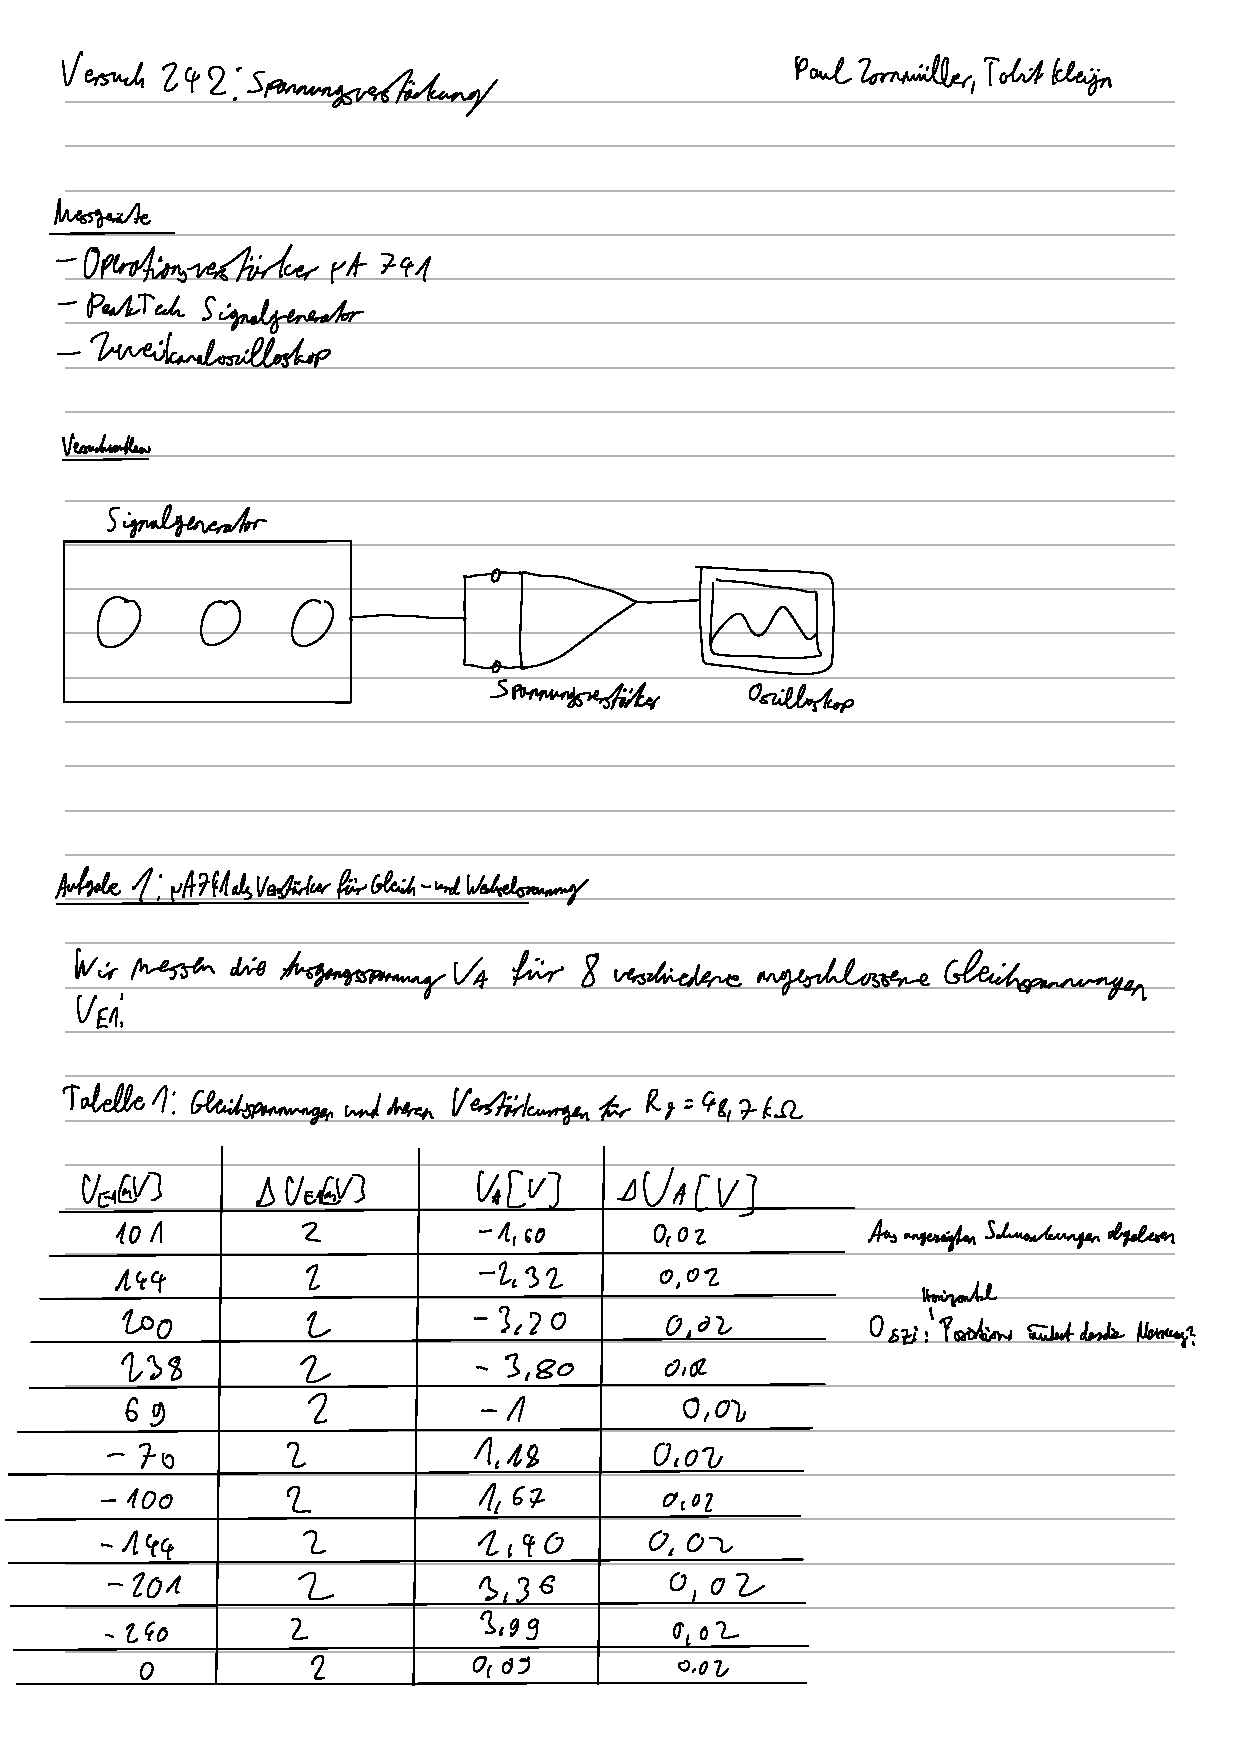
\includepdf[pages=-]{./images/242.pdf}
